% Vorlage für ein Inforz
% Erstellt von: Tobias Otterbein, totterbein@d120.de, Stand: 31.08.2014
% Darf beliebig für ein Inforz angepasst werden.
\documentclass[
    a5paper,
    pagesize,
    twoside,
    fontsize=8pt,
    DIV=15
]{scrreprt}

% Seitenränder festlegen
\usepackage[
    paperheight=214mm,
    paperwidth=152mm,
    left=17mm,
    right=17mm,
    top=17mm,
    bottom=22mm
]{geometry}

% Inforz-Definitionen laden
\usepackage{inforz}

% Pfad für Grafiken festlegen
\graphicspath{{../shared/grafik}}

%Back To The Future Font
\newfont{\bttf}{BTTF scaled 1000}

% Sprache hier einstellen
\usepackage[ngerman]{babel}

\begin{document}
    % Titelseite
    \begin{titlepage}~
    \ThisTileWallPaper{\paperwidth}{\paperheight}{oinforz_cover_ws22}


    \begin{textblock*}{12cm}(1.5cm,1cm)
        
\includegraphics[width=12cm]{inforz_schwarz}
    \end{textblock*}


    \begin{textblock*}{12cm}(1.5cm,19cm)
        %\centering\huge\sffamily\textbf{
        %\textcolor{white}{Willkommen zur Ophase der Fachschaft} \\
        %\textcolor{white}{Informatik im Wintersemester \the\year !}}
    \end{textblock*}

    \begin{textblock*}{7cm}(7cm,5cm)
        \begin{flushright}
            \large\sffamily\textbf{
                \textcolor{.}{Zeitschrift der Studierenden der}\\
                \textcolor{.}{Informatik der TU Darmstadt}}
        \end{flushright}
    \end{textblock*}



    \begin{textblock*}{5cm}(1cm,8cm)
        \begin{rotate}{90}
            \sffamily\huge\textbf{
                \textcolor{.}{Inforz zur Winterophase \the\year}}
        \end{rotate}
    \end{textblock*}


    \begin{textblock*}{2cm}(1cm,12cm)
        \begin{rotate}{90}
            \sffamily\tiny \textcolor{.}{Preis: unbezahlbar}
        \end{rotate}
    \end{textblock*}


    \begin{textblock*}{2cm}(1cm,20cm)
        \begin{rotate}{90}
            \sffamily \textcolor{.}{ISSN: 1614-4295}
        \end{rotate}
    \end{textblock*}
    \begin{tikzpicture}[remember picture,overlay]
        \node[anchor=south] at (current page.south) {
\includegraphics[height=5cm,keepaspectratio]{welcome_winterophase_2223}};
    \end{tikzpicture}
\end{titlepage}
\newpage


    % Stundenplan
    \thispagestyle{empty}
\begin{textblock*}{8cm}(1cm,1cm)
    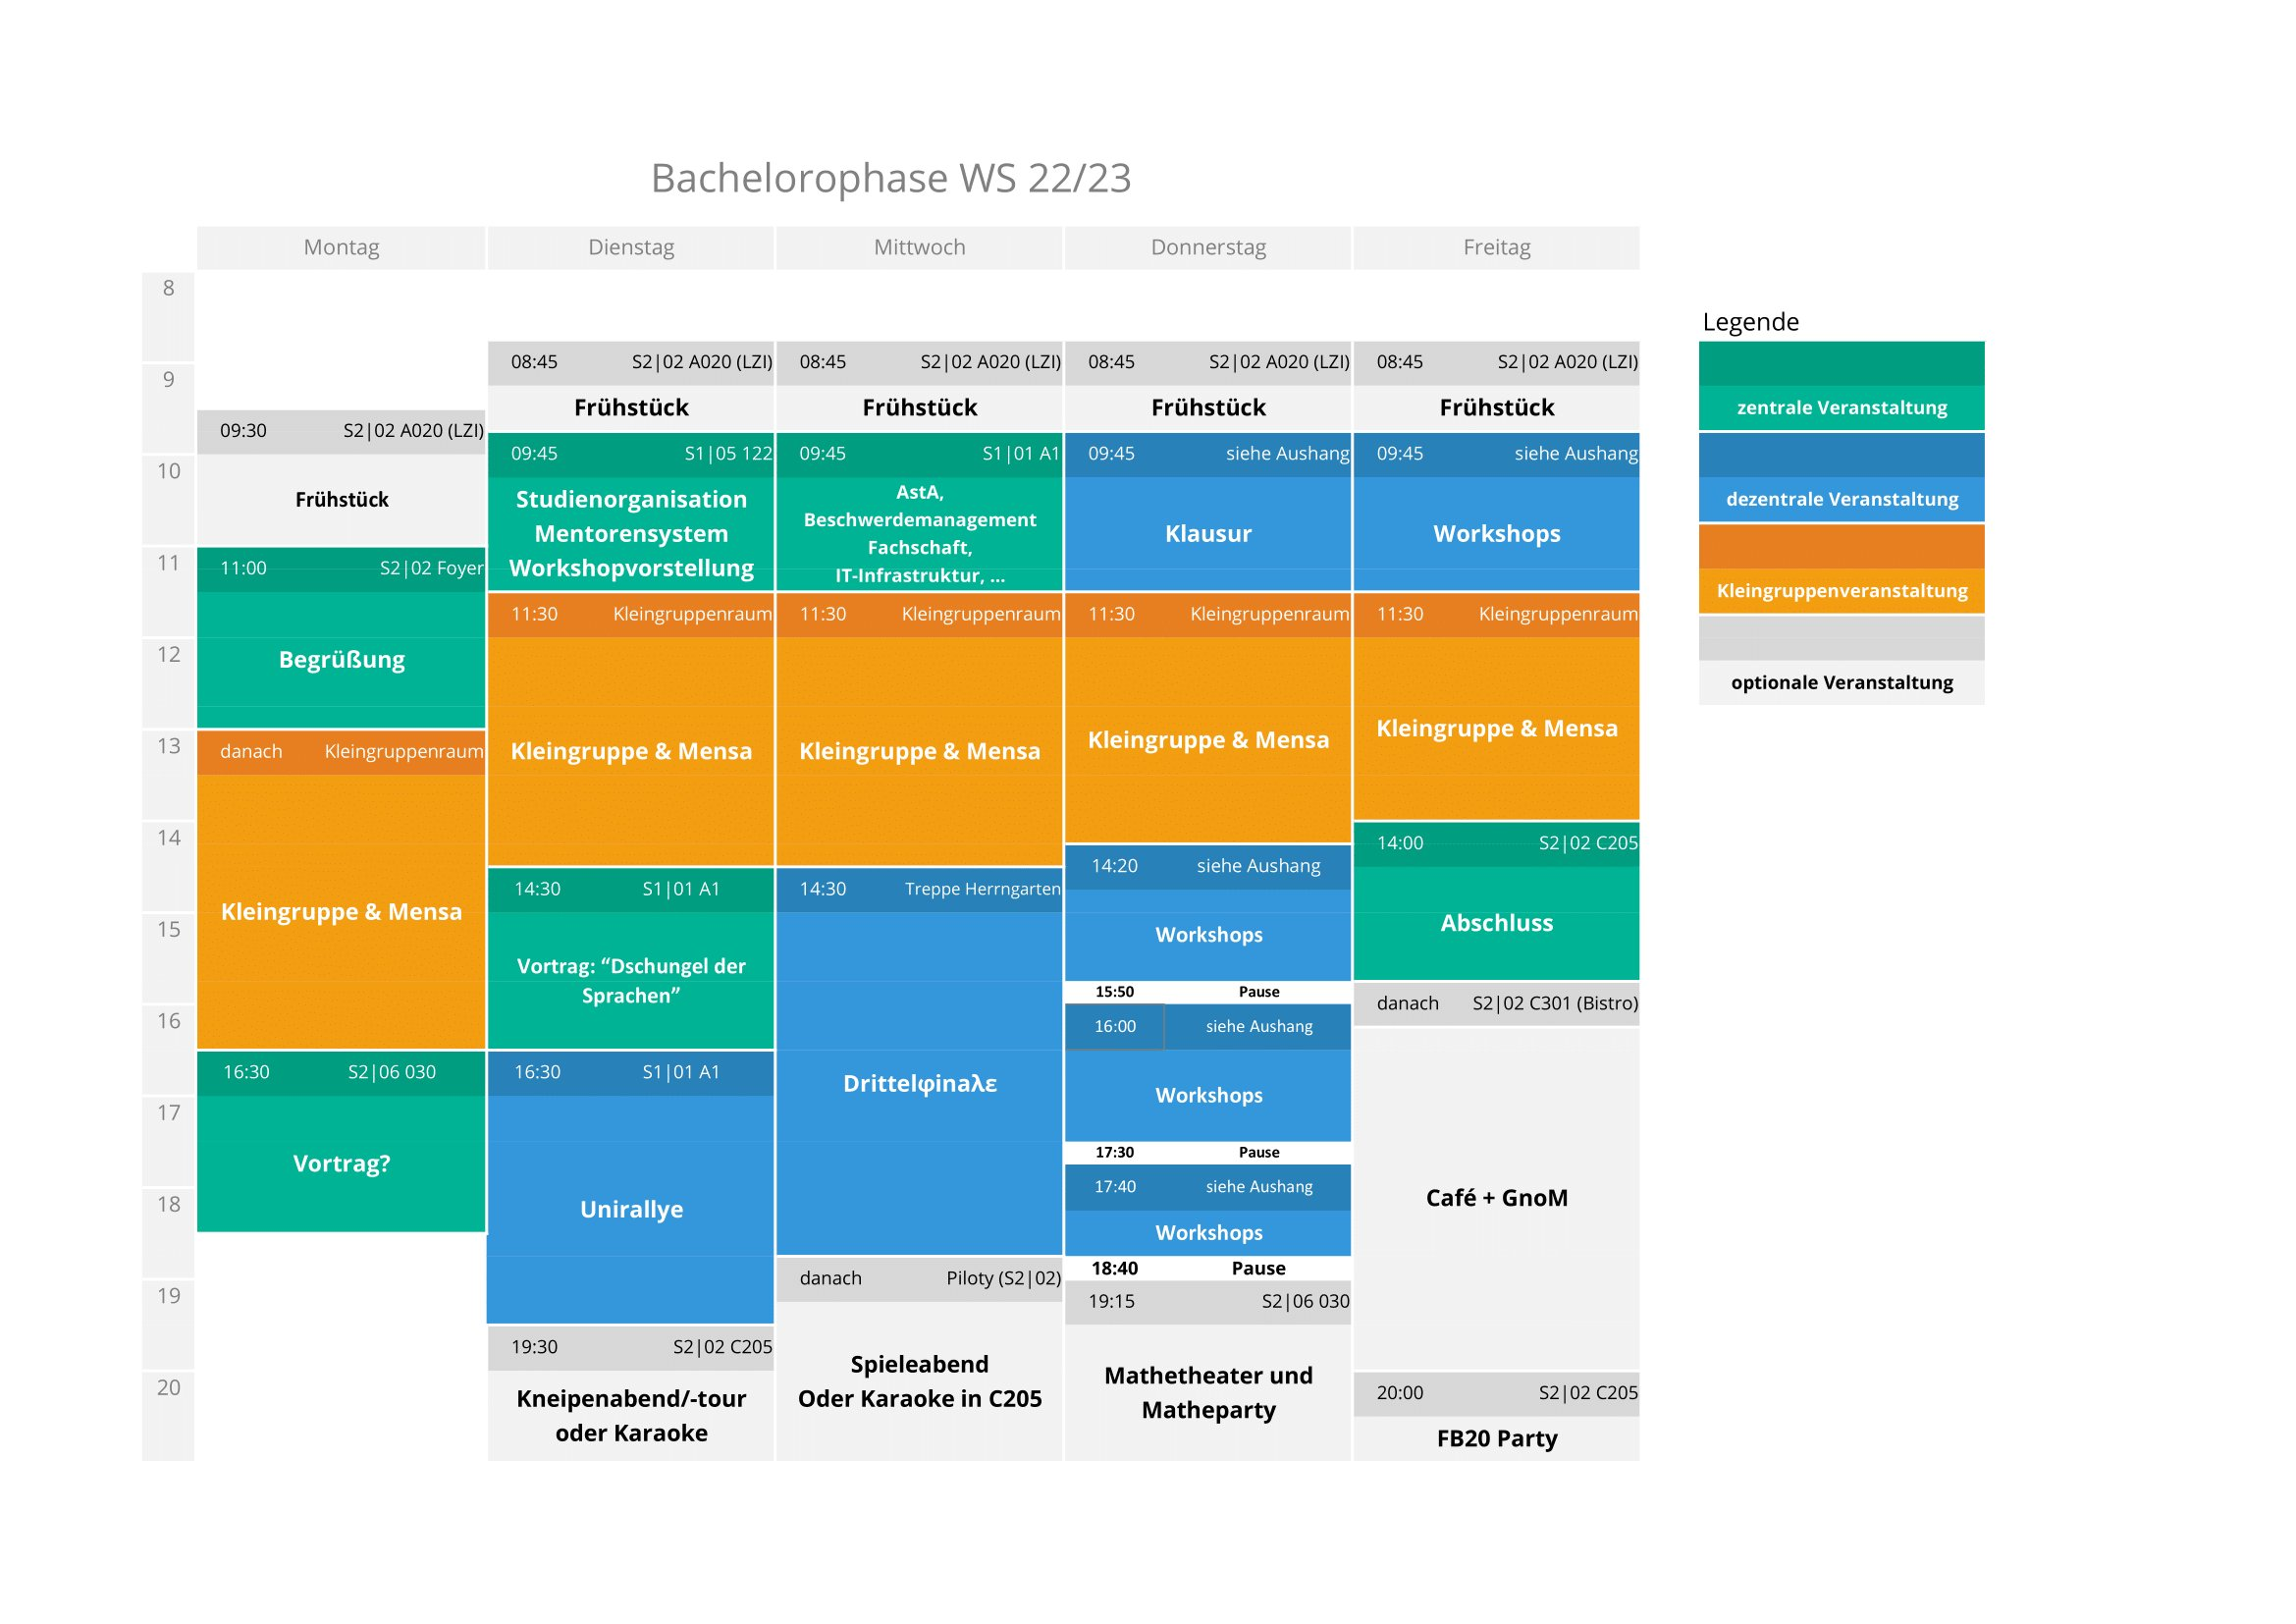
\includegraphics[angle=90,height=15cm]{../grafik/stundenplan}
\end{textblock*}
\cleardoublepage

%\thispagestyle{empty}
%\backgroundsetup{
%scale=1,
%angle=0,
%opacity=1,
%contents={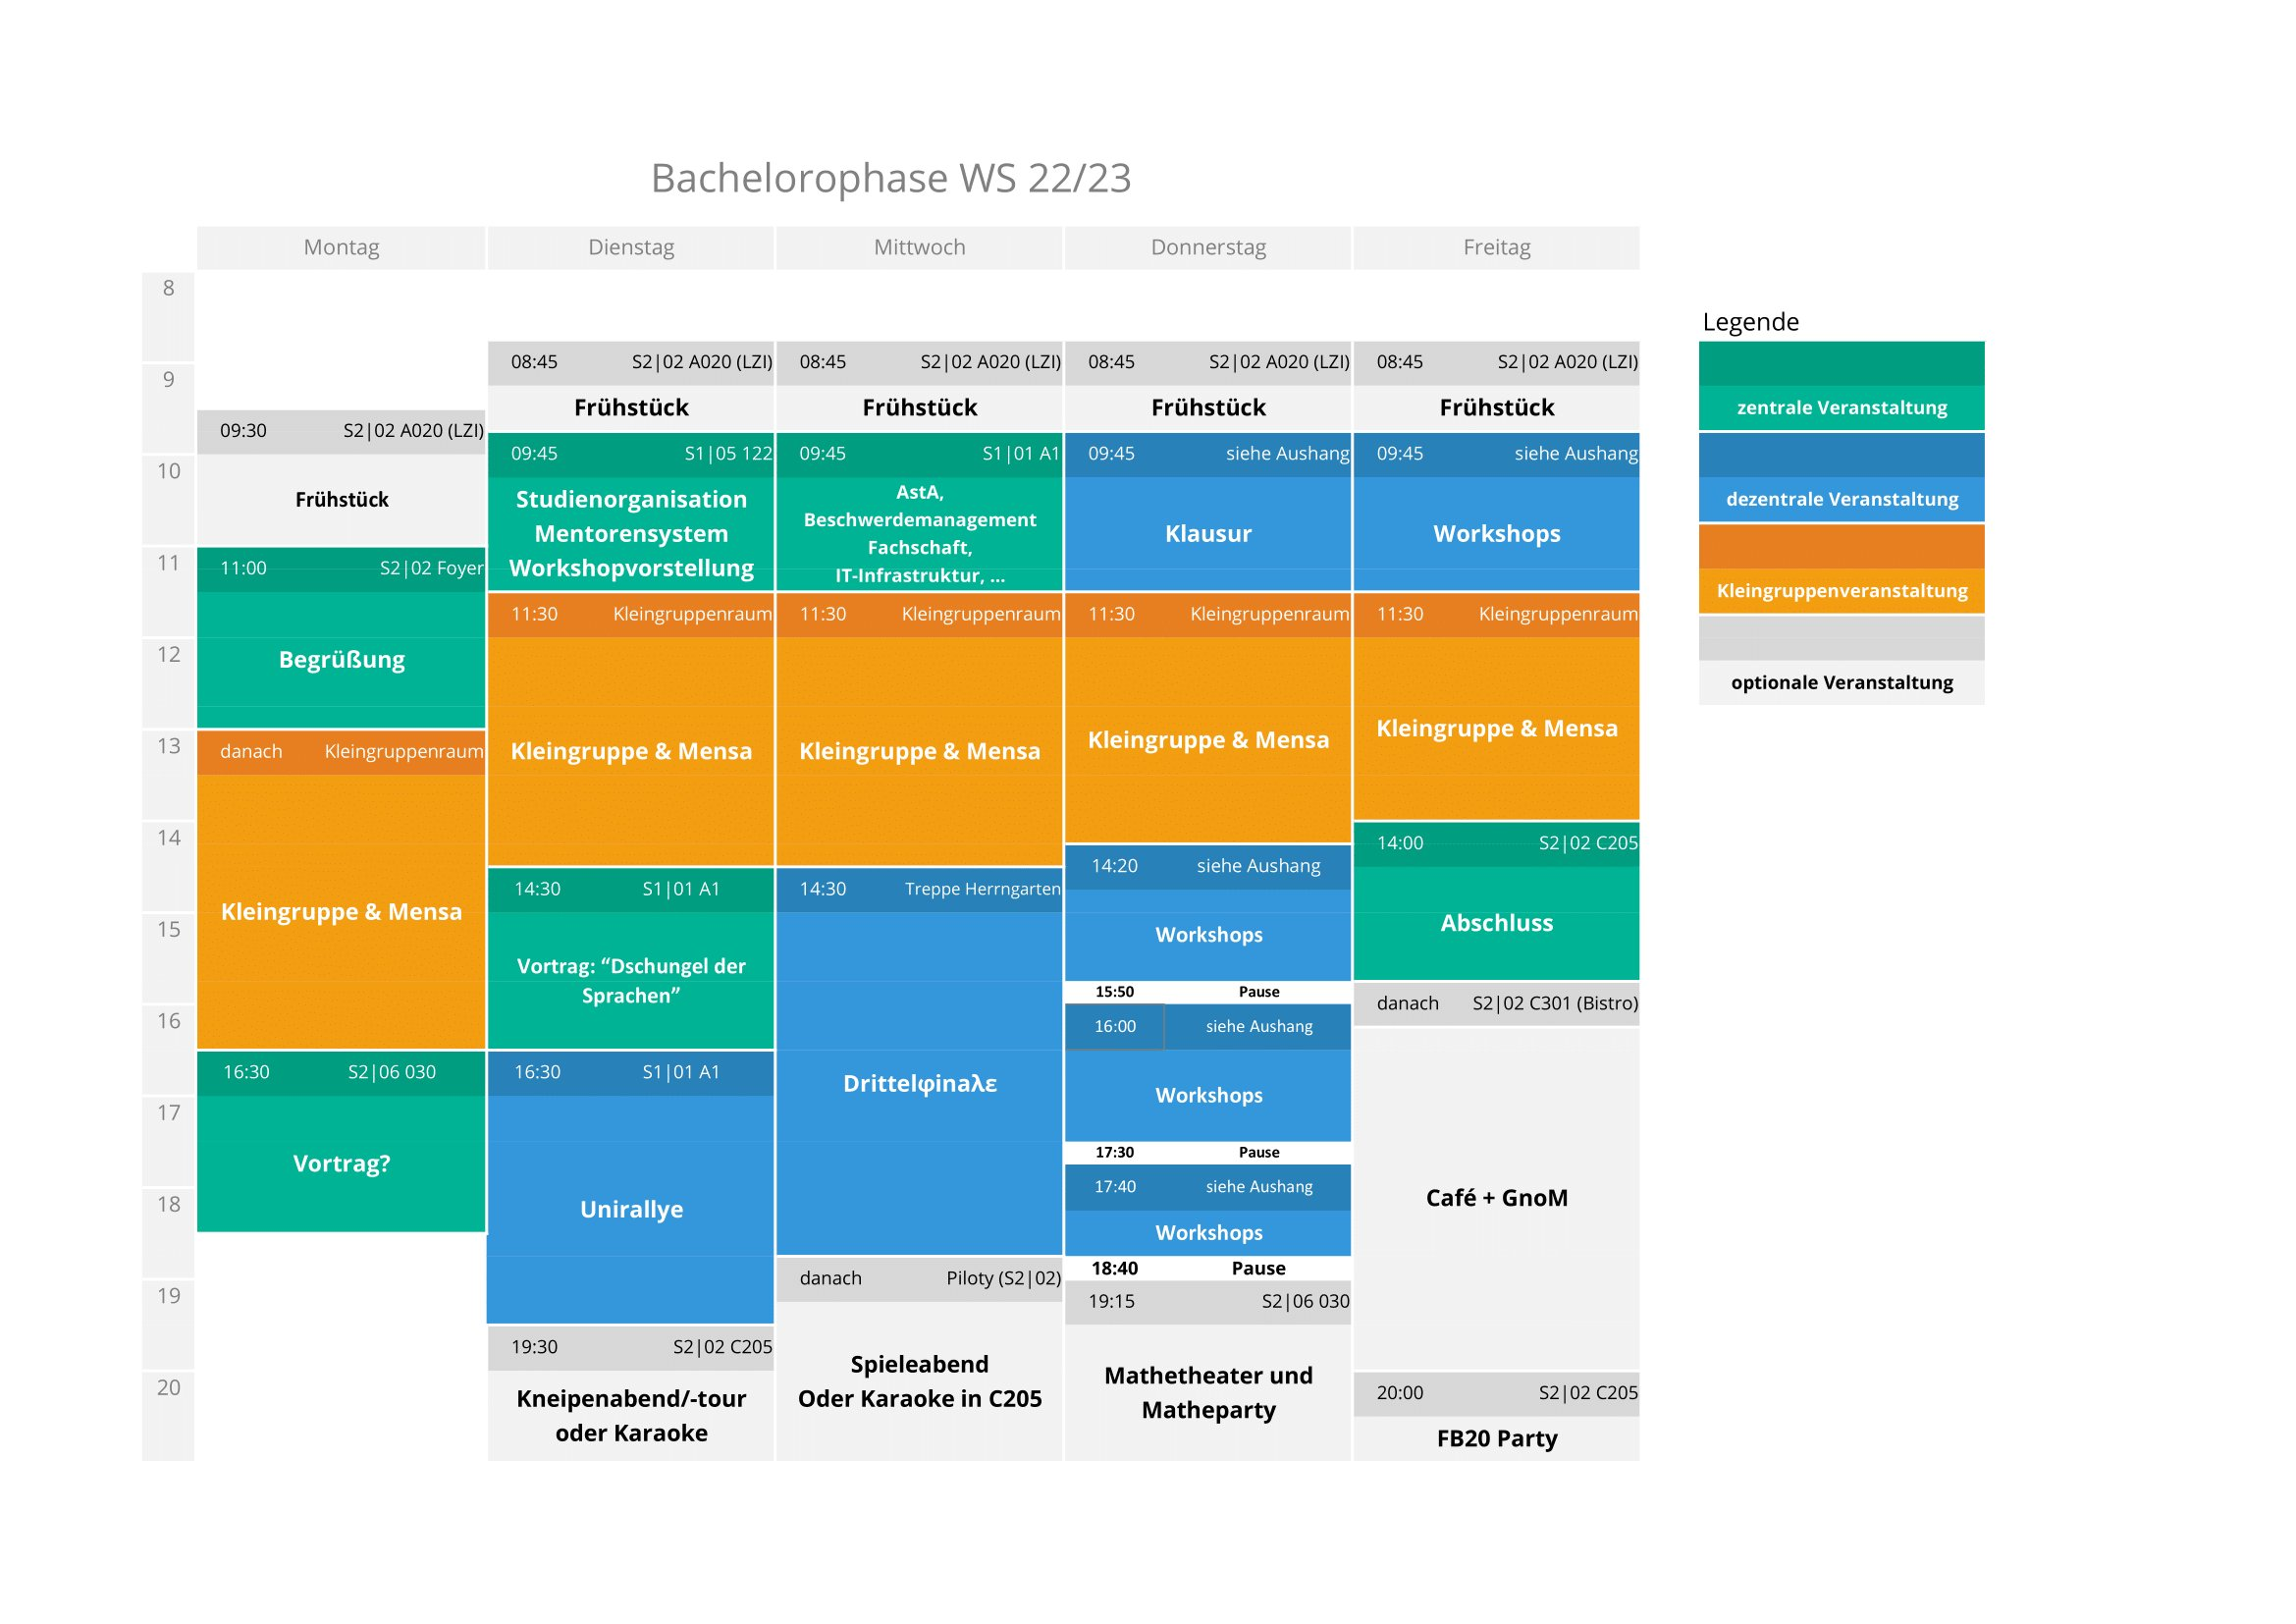
\includegraphics[angle=90, keepaspectratio, height=\paperheight]{../grafik/stundenplan}}
%}

%\cleardoublepage


    % QR-Code
    \artikel*{QR-Code zur Ophasenwebsite}
{Ein QR-Code ist ein zweidimensionaler Code, der mit einem Smartphone gescannt werden kann. Dieser QR-Code enthält einen URL, der direkt auf die Ophasenwebsite verweist.}
{
    \vspace{\fill}
    \begin{figure}[ht!]
        \centering
        \qrcode[hyperlink, height=.5\textwidth]{https://d120.de/ophase}
        \caption*{\large\url{https://d120.de/ophase}\\QR-Code zur Ophasenwebsite}
    \end{figure}
    \vspace{\fill}
}{}

\newpage


    \artikel{Workshops}{Hier finden ihr mehr Informationen über die einzelnen Workshops}{

    \textbf{Jonglieren mit drei Bällen}\\
    In diesem Workshop lernen wir das Jonglieren mit drei Bällen, genauer gesagt das Grundmuster: Die 3-Ball-Kaskade.
    Dies geschieht von Grund auf, wir beginnen mit einem Ball und arbeiten uns dann hoch. Am Ende sollte jeder Teilnehmer die Grundlagen beherrschen
    und in der Lage sein, selbst weiter zu üben. Wer besonders schnell ist, kann auch schon einfachere Tricks ausprobieren oder sogar Vorübungen zu vier Bällen lernen.
    Jonglieren selbst kann als Partytrick, zur Verbesserung von Konzentrationsfähigkeit und dem räumlichen Denkvermögen oder gar als neues Hobby dienen. Ich freue mich auf euch!
    \autor{Nathanael Herwig}

    \textbf{Esperanto}\\
    "Saluton, kara leganto!"
    Am Schreibtisch entworfen, gibt es die Sprache Esperanto seit knapp 130 Jahren. Und doch: Sie lebt und das Konzept einer neutralen Kommunikation auf Augenhöhe begeistert Menschen weltweit. Auch wenn sie heute vorwiegend im kleinen Maßstab angewendet wird, lohnt es sich dieses verbindende Kulturgut zu pflegen. Die klaren Strukturen machen Spaß und bieten einen sanften Einstieg in die Welt der Sprachen. Neben der Einführung in die Grammatik, erwartet euch in diesem Workshop auch ein kleiner Abstecher in die bemerkenswerte Geschichte.
    \autor{Sebastian Bremser}

    \textbf{Mesh-Netzwerke selber bauen}\\
    "Mesh" ist in den letzten Jahren eines der Top-Themen in den Marketingbroschüren und Datenblättern der Routerhersteller geworden. Freifunk ist einer der Pioniere auf dem Gebiet der Entwicklung und dem Aufbau von Mesh-Netzwerken. In diesem Workshop lernst du, wie du dein eigenes, privates Mesh-Netzwerk aufbaust, indem du mit deinen Kommilitonen ein hybrides und verschlüsseltes Mesh-Netzwerk von Grund auf aufbaust.
    \autor{Freifunk Darmstadt}

    \textbf{Blick unter die Haube - PC (de-)montieren und Linux installieren}\\
    Aus welchen Teilen besteht ein PC und wozu sind diese da?

    Im Workshop werden wir in einem kurzen Vortrag die einzelnen Teile eines PCs erläutern. Hands-On wird es Anschauungsobjekte wie geöffnete Festplatten (HDD und SSD), Grafikkarten, CPUs usw. geben.
    Im Anschluss erhalten alle Teilnehmer*innen einen Desktop-PC bei dem Sie RAM und Festplatte  ersetzen und im Anschluss auf dem PC Linux installieren.
    \autor{Stephan Voeth}

    \textbf{Latex}\\
    Hast du schonmal versucht in Office eine richtig komplizierte Formel einzugeben?
    Oder ein Dokument mit vielen Seiten und Bildern genau so zu formatieren, wie eine
    Vorgabe vorgibt? Und plötzlich fällt dir auf, dass du einen Fehler gemacht hast
    und du jetzt bei 50 Überschriften die Schriftgröße anpassen musst? Und am Ende sieht
    plötzlich alles wieder ganz anders aus, sobald du irgendwo eine Zeile änderst oder
    das ganze auf einem anderen Computer öffnest. Zum Glück gibt es etwas, womit das
    viel einfacher geht: LaTeX. Und trotz des komischen Namens wird es auf der ganzen
    Welt von fast allen Wissenschaftlern und von vielen Anderen eingesetzt, wenn sie
    technische oder mathematische Dokumente erstellen. LaTeX ist ein bisschen wie HTML
    und CSS, man schreibt einen reinen Text, versieht ihn mit Markierungen, welcher
    Block welche Rolle hat und kann ihn dann mit speziellen Programmen in formatierte
    Dokumente übersetzen. Klingt nützlich? Ist es auch. Und je eher man anfängt, es zu
    nutzen, desto mehr Ärger kann man sich ersparen. Deshalb bieten wir in diesem Workshop
    einen einfachen und kurzen Einblick. Und irgendwann im Laufe des Studiums braucht
    es sowieso (fast) jeder. Warum also nicht gleich?!


    \textbf{Capture The Flag: Hacking als Wettkampf}\\
    Capture The Flag, oder kurz CTF, sind IT-Security Wettkämpfe über einen begrenzten Zeitraum, bei denen um die Wette gehackt wird.
    Dabei gilt es Aufgaben zu lösen und dadurch Punkte zu gewinnen. Am Ende gewinnt das Team mit den meisten Punkten.

    Die Aufgaben kommen hierbei aus den Bereichen Reverse Engineering, Web Security, Binary Exploitation, Forensik, Kryptographie, Mobile Security und ähnlichem und sind sehr praxisorientiert.

    Wir, das CTF-Team des Darmstädter Chaos Computer Club, wollen euch in diesem Workshop eine hands-on Einführung in dieses Format geben und euch bei euren ersten Flags zur Seite stehen und Fragen beantworten und Hilfestellung geben.
    \autor{Alexander Druffel}

    \textbf{Programmierung von Lego Mindstorms Robotern}\\
    Du hast schon mal ein paar Programmzeilen getippt und willst mal ein bisschen spielerisch testen, ob der Code auch das macht was du willst?
    Hier kannst du einem Lego Mindstorms Roboter programmieren und schon mit wenig Code kleine Aufgaben lösen.
    \autor{David Botschek}

    \textbf{Einstieg in die Entwicklung von Webanwendungen}\\
    Ich möchte den Teilnehmern einen Einblick in die Webentwicklung geben. Dabei gehe ich zuerst auf HTML, Javascript und ein wenig CSS ein und werde dann noch darüber sprechen, wie die Entwicklung mit Framworks und Libraries aussieht. Ziel ist es den Teilnehmern einen groben Überblick über Sprache, Tooling uns sonstiges zu vermitteln.
    \autor{Nicklas Knell}

    \textbf{Studium für Späteinsteiger}\\
    Ich biete einen kleinen Vortrag zum Thema und anschließend einen Workshop für alle, die ein bisschen später zum Studium gefunden haben.
    \autor{Malin Kammer}

    \textbf{Musiknotation und Arrangieren - Einführung in Open-Source-Musiknotation mit MuseScore}\\
    Noten schreiben leicht gemacht! Dieser Workshop richtet sich an alle Studierenden, die Musik schreiben, komponieren, arrangieren oder einfach mal in die Welt der meistgenutzten Open-Source-Musiknotationssoftware MuseScore reinschnuppern wollen. Nach einer kurzen Einführung in das Programm werden wir uns mittels Try-and-Error der Umsetzung Eurer Ideen widmen - Ausprobieren, Arrangieren, Komponieren. Gerne gibt es "Tipps und Tricks der Harmonielehre", den "Unterschied zwischen Tremolo und Triller" oder einen "Crashkurs Bassschlüssel" oben drauf.

    Der Workshop ist auch für Anfänger ausgelegt, es sind keine Vorkenntnisse in der Benutzung von MuseScore nötig. Allerdings solltest du Interesse an Musik haben, rudimentär Noten lesen können und bei dem Wort Andante nicht unbedingt an Nudeln beim Italiener denken.

    Und weil alles mit einem Zitat seriöser wirkt... "Der Takt ist nicht das Zählwerk, sondern der Puls der Musik." (Ulrich Erckenbrecht)
    \autor{Jannis Rösner}

    \textbf{Flaschen-Yoga}\\
    Mehr Bewegung für Informatiker! Wir machen mit euch Yoga für Anfänger - nur anders: Beim Flaschen-Yoga halten wir bei diversen Grundübungen eine offene Flasche in der Hand, die weder abgestellt noch verschüttet werden darf. Austrinken ist jedoch erlaubt. Es macht auf jeden Fall Spaß!
    \autor{Yvonne Meuleneers und Viola Hofmeister}



    \textbf{Einführung in die Hochschulpolitik}\\
    Einführung in die Hochschulpolitik (HoPo 101)

    In einem 10 Minütigen Vortrag kann man nicht vollumfänglich
    über die Hochschulpolitik an der TU Darmstadt aufklären.
    Daher wird dieser Workshop angeboten.

    Ziel ist es die Möglichkeiten studentischer Beteiligung
    sowohl an der Uni (Universitätsversammlung, Senat,...),
    als auch in der studentischen Selbstverwaltung
    (Studierendenparlament, AStA) zu betrachten.
    Damit sollen die Teilnehmenden die Möglichkeit erhalten
    die Politik der Studentischen Gremienmitglieder kritisch
    bewerten zu können oder sogar sofern gewünscht sich
    selbst zu beteiligen.

    Die Workshopleitung ist selbst in der Darmstädter Hochschulpolitik
    aktiv, werden sich jedoch alle Mühe geben, ihre persönliche Meinung
    entssprechend zu kennzeichnen und von Faktenbeschreibungen zu
    trennen.
    \autor{Tobias Huber}

    \textbf{Rugby - Ein Sport für jeden}\\
    Hallo, wir von der Unisportgruppe Rugby wollen euch herzlich an der TU Darmstadt begrüßen und euch unseren Sport näherbringen.
    Dazu laden wir euch in der Herrngarten ein. Dort haben wir für euch ein kleines Programm vorbereitet, das Rugby in jedem Bereich gerecht wird. Unser Sport richtet sich an alle - und damit meinen wir alle. Deswegen kommt vorbei, wir freuen uns auf euch
    \autor{Christoph Schülter}

    \textbf{Codestyle? Warum, läuft doch!}\\
    Tabs oder Spaces, Klammern mit und ohne Leerzeichen, geschweifte Klammern auf der selben oder in der nächsten Zeile: Es gibt sehr viele verschiedene Arten, Code zu formatieren - leider oft auch mehrere verschiedene Formatierungsarten in einem Projekt oder sogar in derselben Datei. Dadurch können sich Bugs besser verstecken und die Zusammenarbeit im Team wird durch unlesbaren Code erschwert.

    Wir zeigen euch, wie ihr euch im Team auf einen gemeinsamen Programmierstil einigen könnt und welche Tools euch dabei helfen, diesen durchzusetzen. So wird das Bearbeiten von komplexen Programmierpraktika für euch leichter und euer Code für die Tutoren besser verständlich.

    Guten Code zeichnet mehr aus, als fehlerfrei und kompakt zu sein. Code muss sich selbst dokumentieren und wartbar sein. Nur dann ist eine gemeinsame Entwicklung in Projekten möglich.
    \autor{Pickware GmbH}

    \textbf{Stundenplanerstellung und Informations-/ Fragerunde für alle "Nicht-Bachelor of Science-Studiengänge"}\\
    Dieser Workshop soll eine Möglichkeit bieten, den Student*innen, welche nicht im Bachelor of Science studieren, offengebliebene Fragen zu beantworten, beim Erstellen der Stundenpläne zu helfen, generelle Hilfestellungen zu geben, oder sich unter den Hunderten von Ersties auch einfach mal zu sehen und zu wissen, dass es noch andere mit dem selben Studiengang gibt.
    \autor{Dini \& Guido (vermutlich auch ein Assitent von Hr. Gallenbacher)}
}{}


    % Rückseite
    \thispagestyle{empty}
\ThisCenterWallPaper{0.9}{../grafik/lageplan_mit_markierungen}

\begin{textblock*}{10cm}(7mm,6mm)
    \normalsize \textbf{Dieses Inforz gehört:}
\end{textblock*}

\begin{textblock*}{4cm}(10cm,1cm)
    
\includegraphics[width=4cm]{../grafik/wesen/wesen_uni}
\end{textblock*}


\end{document}
